\chapter{Regions of interest}

The regions of interest was chosen to get a full representation of the hand, to investigate the region that shows the most significant difference when computing the statistical test. 
Regions in the nail folds is often used to access the microcirculatory hemodynamics \cite{martina1998}. This region should therefore be expected to give some information on the changes in the capillaries which can be an effect of vasomotion. 

To better choose the regions of interest the original image was converted to a gray scale image to get better contrast in the image, this can be seen in \ref{fig:mat2grayHand}. 

\begin{figure}[H]
	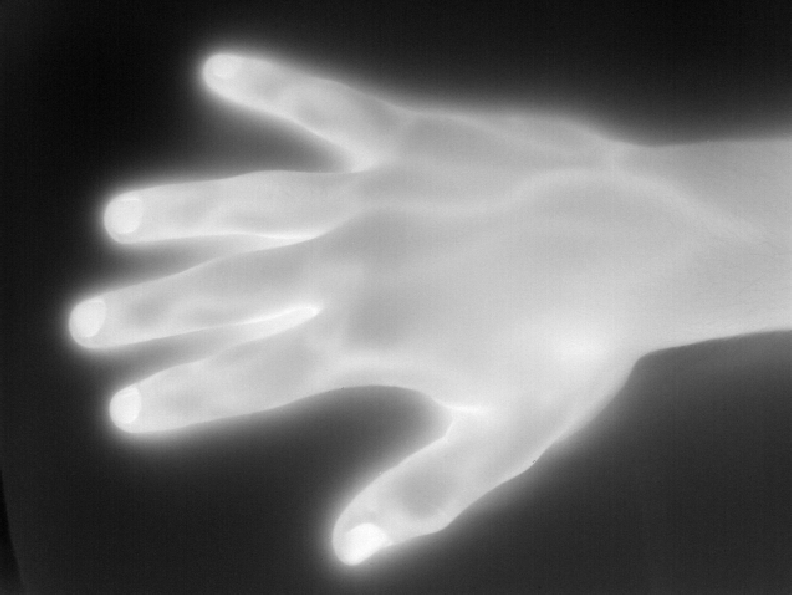
\includegraphics[width=0.6\textwidth]{figures/mat2grayHand}  %<--but is not needed.
	\caption{Image of frame number one for a subject, mat2gray image}
	\label{fig:mat2grayHand}  %<--give the figure a label, so you can reference!
\end{figure}

28 regions on the hand was chosen illustrated on \ref{fig:roiHand}, starting from the fingertips and elongating down the hand to the beginning of the wrist. Each region gives an pixelintensity value from one pixel. The mean of the chosen pixel value and the neighbor pixels, a total  of nine pixels, is calculated for each region to get a more general value for the specific region.

\begin{figure}[H]
	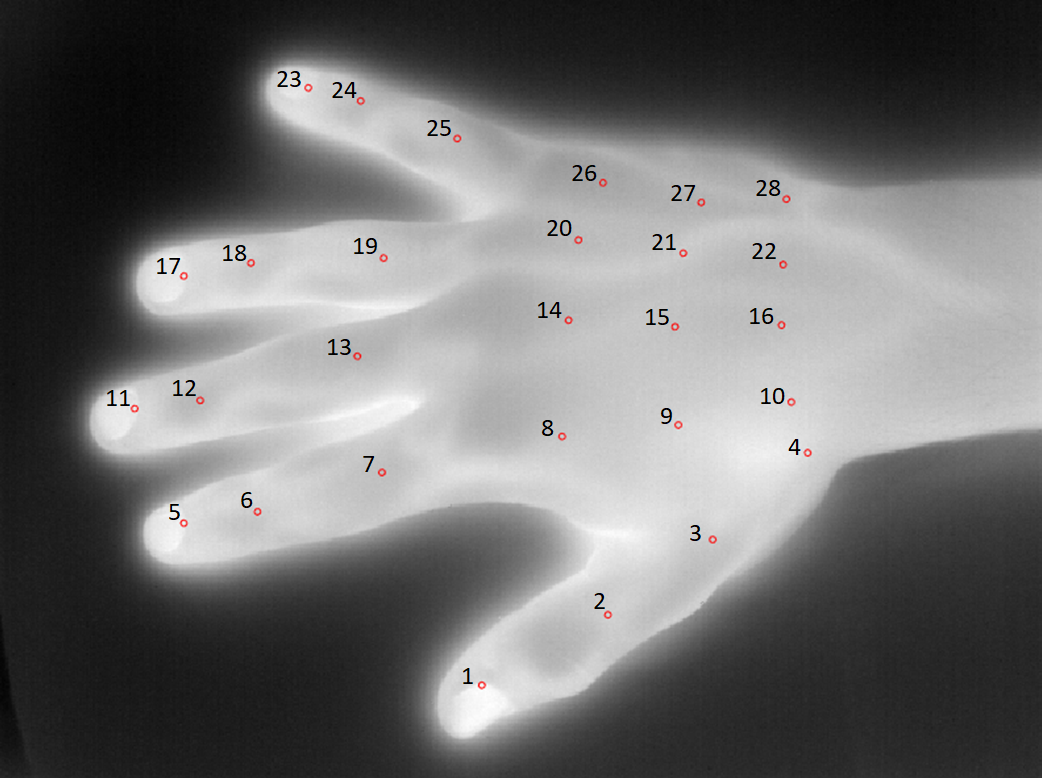
\includegraphics[width=0.6\textwidth]{figures/roiHand}  %<--but is not needed.
	\caption{Image of frame number one for a subject, with regions of interest plottet on 28 areas of the hand}
	\label{fig:roiHand}  %<--give the figure a label, so you can reference!
\end{figure}

The regions is constant for all frames, assuming that the subject was sitting still under the whole measurement
The regions accounts for both the uncuffed and cuffed conditions for each subject, assuming that the position of the hand was at the same position in both conditions. 
The regions was chosen for each subject by looking at the first frame and finding the coordinates of the center pixel in Matlab. 


% The tex should be seen on as fast written worksheets, so some elaboration is needed.